% !TEX root = ../chem_ia.tex
\section{Methodology}

\subsection{Apparatus}

\begin{table}[h!]
\centering

\begin{tabular}{m{5cm} m{5cm} m{4cm}} 
 \toprule
 Chemicals & Glassware & Miscellaneous \\
 \midrule
	\begin{itemize}[]
	  \item $120$ $cm^3$ $1 M$ $HCl$
	  \item $120$ $cm^3$ $4 M$ $Acetone$
	  \item $120$ $cm^3$ $.005 M$ $I_2$ solution 
	  \item $165$ $cm^3$ Distilled $H_2O$
	\end{itemize} & 
	\begin{itemize}[]
	  \item $100$ $mL$ Erlenmeyer Flask
	  \item $1000$ $mL$ Beaker
	  \item $10$ $mL$ Graduated Cylinder
	  \item Test Tube(s)
	\end{itemize} & 
	\begin{itemize}[]
	  \item Ice
	  \item Thermometer
	  \item Ring Stand
	  \item Poly Water Bath
	  \item $2x$ Beaker Clamp
	  \item Water Source
	\end{itemize} \\
  \bottomrule
\end{tabular}
\caption{Materials}
\label{table:apparatus}
\end{table}

\subsection{Experimental Procedure}
\subsubsection{Rate Law Determination}
	\begin{enumerate}[itemsep=-1ex]
	  \item Prepare a water bath at room temperature in a $1000$ $mL$ beaker.
	  \item Clamp a $100$ $mL$ erlenmeyer flask and a separate test tube into the water bath.
	  \item Measure out the appropriate amounts of $HCl$, $Acetone$, and $H_2O$ (as listed in \cref{table:1_config}) into the $10$ $mL$ graduated cylinder and add these substances to the clamped erlenmeyer flask.
	  \item Measure out the appropriate amount of $I_2$ (as listed in \cref{table:1_config}) into the $10$ $mL$ graduated cylinder and pour into the clamped test tube.
	  \item Ensure that the the reactants in the test tube and flask are fully immersed in the water bath and allow 5 minutes for temperature equilibrium to be reached.
	  \item Record the water bath temperature after this period is complete. Attempt to maintain this temperature for all trials to limit potential confounding results for rate law determination.
	  \item Remove the test tube containing the iodine solution and immediately add its contents to the flask containing $HCl$, $Acetone$, and $H_2O$, starting a timer after the addition.
	  \item Swirl the reaction mixture by gently swirling the ring for $30$ $s$ and then allow the solution to sit.
	  \item When the iodine color (brownish-red) has completely disappeared, stop the timer and record the total reaction time (as the reaction is complete).
	  \item Clean the glassware thoroughly and dry (it is not necessary to clean the test tube as it will always contain iodine solution with a constant concentration).
	  \item Repeat steps 2-10 two more times for configuration $\#1$ in \cref{table:1_config}.
	  \item Repeat steps 2-11 for all remaining configurations in \cref{table:1_config}.
	  \item Thoroughly clean all glassware and dispose of any leftover products/substances safely.
	\end{enumerate}

\subsubsection{Activation Energy Determination}
	\begin{enumerate}[itemsep=-1ex]
	  \item Prepare a water bath at temperature within the range listed in \cref{table:2_config} either in the Pro Water Bath (for high temperatures) or in a $1000$ $mL$ beaker with ice (for the low temperature).
	  \item Clamp a $100$ $mL$ erlenmeyer flask and a separate test tube into the water bath.
	  \item Measure out the appropriate amounts of $HCl$, $Acetone$, and $H_2O$ (as listed in \cref{table:2_config}) into the $10$ $mL$ graduated cylinder and add these substances to the clamped erlenmeyer flask.
	  \item Measure out the appropriate amount of $I_2$ (as listed in \cref{table:2_config}) into the $10$ $mL$ graduated cylinder and pour into the clamped test tube.
	  \item Extra care should be taken to measure out exact volumes of the reactants, as they must be controlled for accurate determination of temperature-dependence on the rate constant.
	  \item Ensure that the the reactants in the test tube and flask are fully immersed in the water bath and allow 5 minutes for temperature equilibrium to be reached.
	  \item Record the water bath temperature after this period is complete.
	  \item Remove the test tube containing the iodine solution and immediately add its contents to the flask containing $HCl$, $Acetone$, and $H_2O$, starting a timer after the addition.
	  \item Swirl the reaction mixture by gently swirling the ring for $30$ $s$ and then allow the solution to sit.
	  \item When the iodine color (brownish-red) has completely disappeared, stop the timer and record the total reaction time (as the reaction is complete).
	  \item Clean the glassware thoroughly and dry (it is not necessary to clean the test tube as it will always contain iodine solution with a constant concentration).
	  \item Repeat steps 2-11 two more times for temperature $\#1$ in \cref{table:2_config}.
	  \item Repeat steps 2-12 for all remaining temperature ranges in \cref{table:2_config}.
	  \item Thoroughly clean all glassware and dispose of any leftover products/substances safely.
	\end{enumerate}

\begin{table}[!htb]
    \begin{minipage}{.5\linewidth}
      \caption{Rate Law Experiment}
      \centering
		\begin{tabular}{|c|c|c|c|c|} 
		 \hline
		 \multicolumn{5}{|c|}{Volumes $(mL)$} \\
		 \hline
		$HCl$ & $Acetone$ & $I_2$ & $H_2O$ & Total \\
		  \hline
		  $5$ & $5$ & $5$ & $10$ & $25$ \\
		  \hline
		  $5$ & $5$ & $10$ & $5$ & $25$ \\
		  \hline
		  $5$ & $10$ & $5$ & $5$ & $25$ \\
		  \hline
		  $10$ & $5$ & $5$ & $5$ & $25$ \\
		  \hline
		\end{tabular}
		\label{table:1_config}
    \end{minipage}%
    \begin{minipage}{.5\linewidth}
      \centering
        \caption{Activation Energy Experiment}
		\begin{tabular}{|c|c|c|c|c|c|} 
		 \hline
		  \multirow{2}{*}{Temperature $(\degree C)$} & \multicolumn{5}{c|}{Volumes $(mL)$} \\
		  	\cline{2-6}
		 	& $HCl$ & $Acetone$ & $I_2$ & $H_2O$ & Total \\
		  \hline
		  $10-15$ & $5$ & $5$ & $5$ & $10$ & $25$ \\
		  \hline
		  $30-35$ & $5$ & $5$ & $10$ & $5$ & $25$ \\
		  \hline
		  $40-45$ & $5$ & $10$ & $5$ & $5$ & $25$ \\
		  \hline
		\end{tabular}
		\label{table:2_config}
    \end{minipage}
    \caption{Experimental Configurations}
    \label{table:config}
\end{table}

\subsection{Risk Assessment}

\begin{enumerate}[label=(\alph*),itemsep=-1ex]
	\item \textbf{Experimental Safety}
		\begin{enumerate}[label=(\roman*)]
			\item Acetone is highly flammable and can cause moderate irritation on repeated exposure to skin. Hydrochloric acid is corrosive and can lead to severe damage to both the eyes and skin in the case of direct contact. Strong iodine solution is partially corrosive and can cause blistering or necrosis of the skin on direct contact~\parencite{acetone, acid, iodoacetone}. To counteract these potential concerns, an apron and goggles were worn for the duration of the experiment. All materials were kept at a moderate distance from the body and spills were immediately cleaned.
			\item Glassware is relatively fragile and any potential breakage can be harmful to those in the lab, both through glass shards and substance spillage. To remedy, extreme caution is used at all times in the lab, especially when handling glassware. In the case that glass did break, the teacher would immediately assist in disposing of any pieces prior to the resumption of the experiment. 
			\item Hot water or glassware can cause sudden reactions and burns of the skin. As water was heated and glassware (with various chemicals) were placed in the water baths, tongs were used at all times to handle warm glass. The water was never directly touched and the water bath was kept closed when not in use.
		\end{enumerate}
	\item \textbf{Environmental Concerns}
	\begin{itemize}[label={}]
	  \item All materials were properly stored and disposed of based on lab best practices and teacher advice to prevent any potential environmental contamination. No limited resources were used nor were any harmful byproducts produced.
	\end{itemize}
	\item \textbf{Ethical Concerns}
	\begin{itemize}[label={}]
	  \item Materials were measured out in small quantities to minimize the potential wastage of any chemicals. No live organisms were employed, so limited ethical concerns were present.
	\end{itemize}
\end{enumerate}

% !TEX root = ../chem_ia.tex
\begin{figure}[!htb]
    \centering
    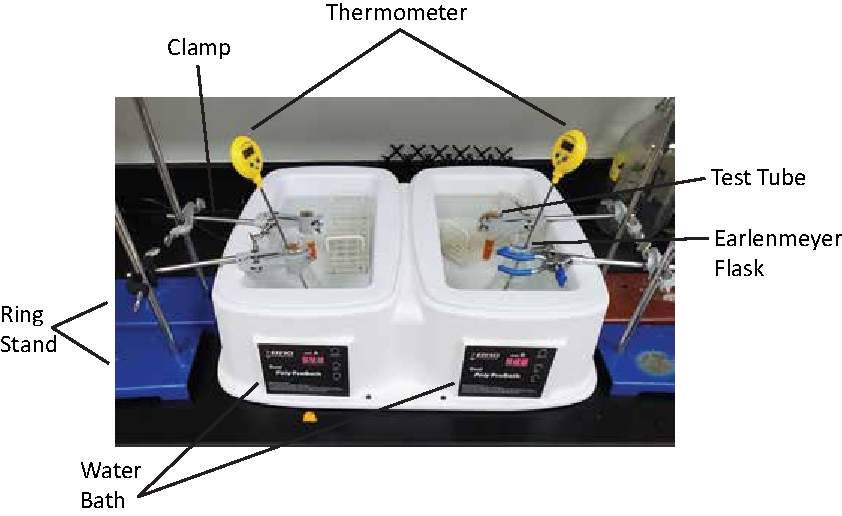
\includegraphics[width=.8\textwidth]{fig/images/visual_setup.pdf}
    \caption{Labelled image depicting the visual setup of the experiment being conducted for two different temperatures.}
    \label{fig:visual_setup}
\end{figure}